%!TEX root = ../thesis.tex

\section{Introduction}
% Introduction to the general topic of GW
In 1916, Einstein predicted the existence of gravitational waves (GW). Nearly
100 years later, on September 14, 2015, the first detection of a gravitational
wave\cite{PhysRevLett.116.061102}, emitted by two merging black holes, confirmed
his prediction. This detection marked the beginning of the GW astronomy era.
Until then, it was also the last missing extrasolar messenger needed for 
full-scale multi-messenger physics.
\cite{Branchesi_2016} 

% Multi-Messenger physics: Importance of latency
Because multi-messenger physics utilizes different messengers to observe the 
same transient, it is of paramount interest to minimize the latency between 
the detector measuring the GW and its reported detection. This allows for
fast follow-up observations of the other messengers.

% Descibe the current situation: We have several detectors. The measurement is
% noisy.
When analyzing the \textit{strain} $h(t)$ measured by the detector, the
fundamental assumption is that it is made up by the GW \textit{signal} $s(t)$
and \textit{noise} $n(t)$ whereas

\begin{equation}
  h(t) = n(t) + s(t)
\end{equation}

Analyzing $h(t)$ about the possible occurence of $s(t)$ is currently done by
using an approach called matched filtering. Matched filtering works by 
convoluting precalculated models of expected signals, so called templates, with
the measured data generating a signal-to-noise (SNR) time series. Because the
parameters of the expected signals are not known in advance, the template bank
spans a large astronomical parameter space.
Using a SNR threshold, we can extract \textit{triggers} indicating possible GW 
signals. Clustering together close triggers leads to a \textit{candidate event}.

Convoluting the measured data with the whole template bank is computationally
expensive, which in turn leads to a high latency between data aggregation and
the reported detection. This motivates the search for methods which are less
computationally expensive and thus provide a low-latency detection algorithm.

\begin{figure}[ht]
  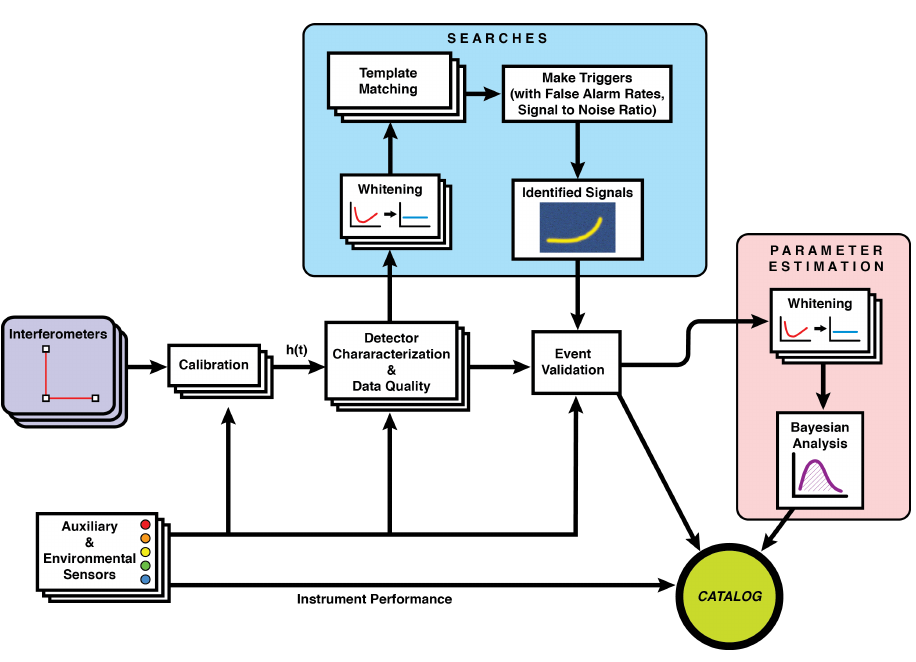
\includegraphics[width=0.95\textwidth]{img/1_introduction/data_processing.png}
  \caption{A simplified schematic summarizing the main steps in LIGO-Virgo data
           processing, from the output of the data to the results reported in a
           catalog of transient events.}
  \label{fig:1_data_processing}
  \centering
\end{figure}

In \autoref{fig:1_data_processing}, taken from \cite{2020CQGra..37e5002A},
we can see a simplified schematic summarizing the main steps in LIGO-Virgo data
processing. The detectors are highly sensitive which makes them prone to
different noise sources. One observed phenomenon are so called glitches which
can mimic true transient astrophysical signals \cite{2020CQGra..37e5002A}.
After a quality control, the data is being searched for GW signals and in case
a signal is found i.e. an candidate event, the parameters are being estimated.

Each candidate event gets a statistical significance assigned, which is given by the 
\textit{false-alarm rate} (FAR) of the search.\cite{2020CQGra..37e5002A} The FAR is
basically telling us how many \textit{false positives}
occured over the duration of the analyzed data. To count the amount of
false positives, we use the ranking statistic, given by the maximal SNR
of the considered candidate event, as the threshold. Current low-latency searches
do not distribute any event candidates with a FAR greated than 1 per month.
\cite{PhysRevD.98.024050}

In their pioneering works, \citeauthor{PhysRevD.97.044039} \cite{PhysRevD.97.044039}
and \citeauthor{PhysRevLett.120.141103} \cite{PhysRevLett.120.141103} showed
that \textit{convolutional neural networks} (CNN) can be used to distinguish 
pure noise from noise containing a GW signal. Both works use a classical binary
classification framework where they utilize the \textit{false alarm probability}
(FAP) to compare their results to matched filtering. Applying matched filtering
on fixed sized samples to compute the FAP and using it to compare the two
approaches is problematic because the matched filtering approach used in the 
LIGO-Virgo data processing pipeline acts on a time series of arbitrary length
resp. on a continous data stream. \cite{PhysRevD.100.063015}
While training a neural network (NN) is also rather computationally expensive, the
evaulation of a trained NN can be done in a fraction of a second. Being able
to easily continue the training of the NN on new detections might proof to
be another advantage.

In this thesis, we will use a similar \textit{deep learning} (DL) approach to search
for simulated GW signals injected in simulated gaussian noise. While working on
this thesis, a heavy focus was put on exploring the space of analyzing GW using
DL approaches. This lead to a rather general approach in the codebase which
should make it easily extenable.

This thesis is organized as follows. In Section 2 we first establish the data
used for our DL approach and how it is being generated. In section 3 
we will describe the actual DL approach as well as its implementation.
In section 4 results are being discussed.
